% ICCV 2025 Paper Template

\documentclass[10pt,twocolumn,letterpaper]{article}

%%%%%%%%% PAPER TYPE  - PLEASE UPDATE FOR FINAL VERSION
% \usepackage{iccv}              % To produce the CAMERA-READY version
\usepackage[review]{iccv}      % To produce the REVIEW version
% \usepackage[pagenumbers]{iccv} % To force page numbers, e.g. for an arXiv version

% Import additional packages in the preamble file, before hyperref
%
% --- inline annotations
%
\newcommand{\red}[1]{{\color{red}#1}}
\newcommand{\todo}[1]{{\color{red}#1}}
\newcommand{\TODO}[1]{\textbf{\color{red}[TODO: #1]}}
% --- disable by uncommenting  
% \renewcommand{\TODO}[1]{}
% \renewcommand{\todo}[1]{#1}



% It is strongly recommended to use hyperref, especially for the review version.
% hyperref with option pagebackref eases the reviewers' job.
% Please disable hyperref *only* if you encounter grave issues, 
% e.g. with the file validation for the camera-ready version.
%
% If you comment hyperref and then uncomment it, you should delete *.aux before re-running LaTeX.
% (Or just hit 'q' on the first LaTeX run, let it finish, and you should be clear).
\definecolor{iccvblue}{rgb}{0.21,0.49,0.74}
\usepackage[pagebackref,breaklinks,colorlinks,allcolors=iccvblue]{hyperref}
\usepackage{xcolor}
\usepackage{lipsum}
\usepackage{booktabs}
\usepackage{graphicx}
\usepackage{colortbl}
\usepackage{makecell}
%%%
\usepackage{arydshln} % For dashed lines
\definecolor{lightgray}{rgb}{0.7,0.7,0.7} % Adjust RGB for lighter dashed lines
\usepackage{multirow}

\usepackage{xr}
\externaldocument[art1-]{supplement}


\newcommand{\filler}[1]{\textcolor{blue}{filler: #1}}
\newcommand{\sv}[1]{\textcolor{brown}{SV: #1}}

\newcommand{\wzy}[1]{{\color{violet}{\bf{[WZY: #1]}}}}
\newcommand{\shijie}[1]{\textcolor{orange}{Shijie: #1}}

%%%%%%%%% PAPER ID  - PLEASE UPDATE
\def\paperID{5678} % *** Enter the Paper ID here
\def\confName{ICCV}
\def\confYear{2025}

%%%%%%%%% TITLE - PLEASE UPDATE
\title{VLM4D: Towards Spatiotemporal Awareness in Vision Language Models
}

%%%%%%%%% AUTHORS - PLEASE UPDATE
\author{First Author\\
Institution1\\
Institution1 address\\
{\tt\small firstauthor@i1.org}
% For a paper whose authors are all at the same institution,
% omit the following lines up until the closing ``}''.
% Additional authors and addresses can be added with ``\and'',
% just like the second author.
% To save space, use either the email address or home page, not both
\and
Second Author\\
Institution2\\
First line of institution2 address\\
{\tt\small secondauthor@i2.org}
}

\begin{document}
% \maketitle
\twocolumn[{%
\renewcommand\twocolumn[1][]{#1}%
\maketitle
    \captionsetup{type=figure}
    \vspace{-9mm}
    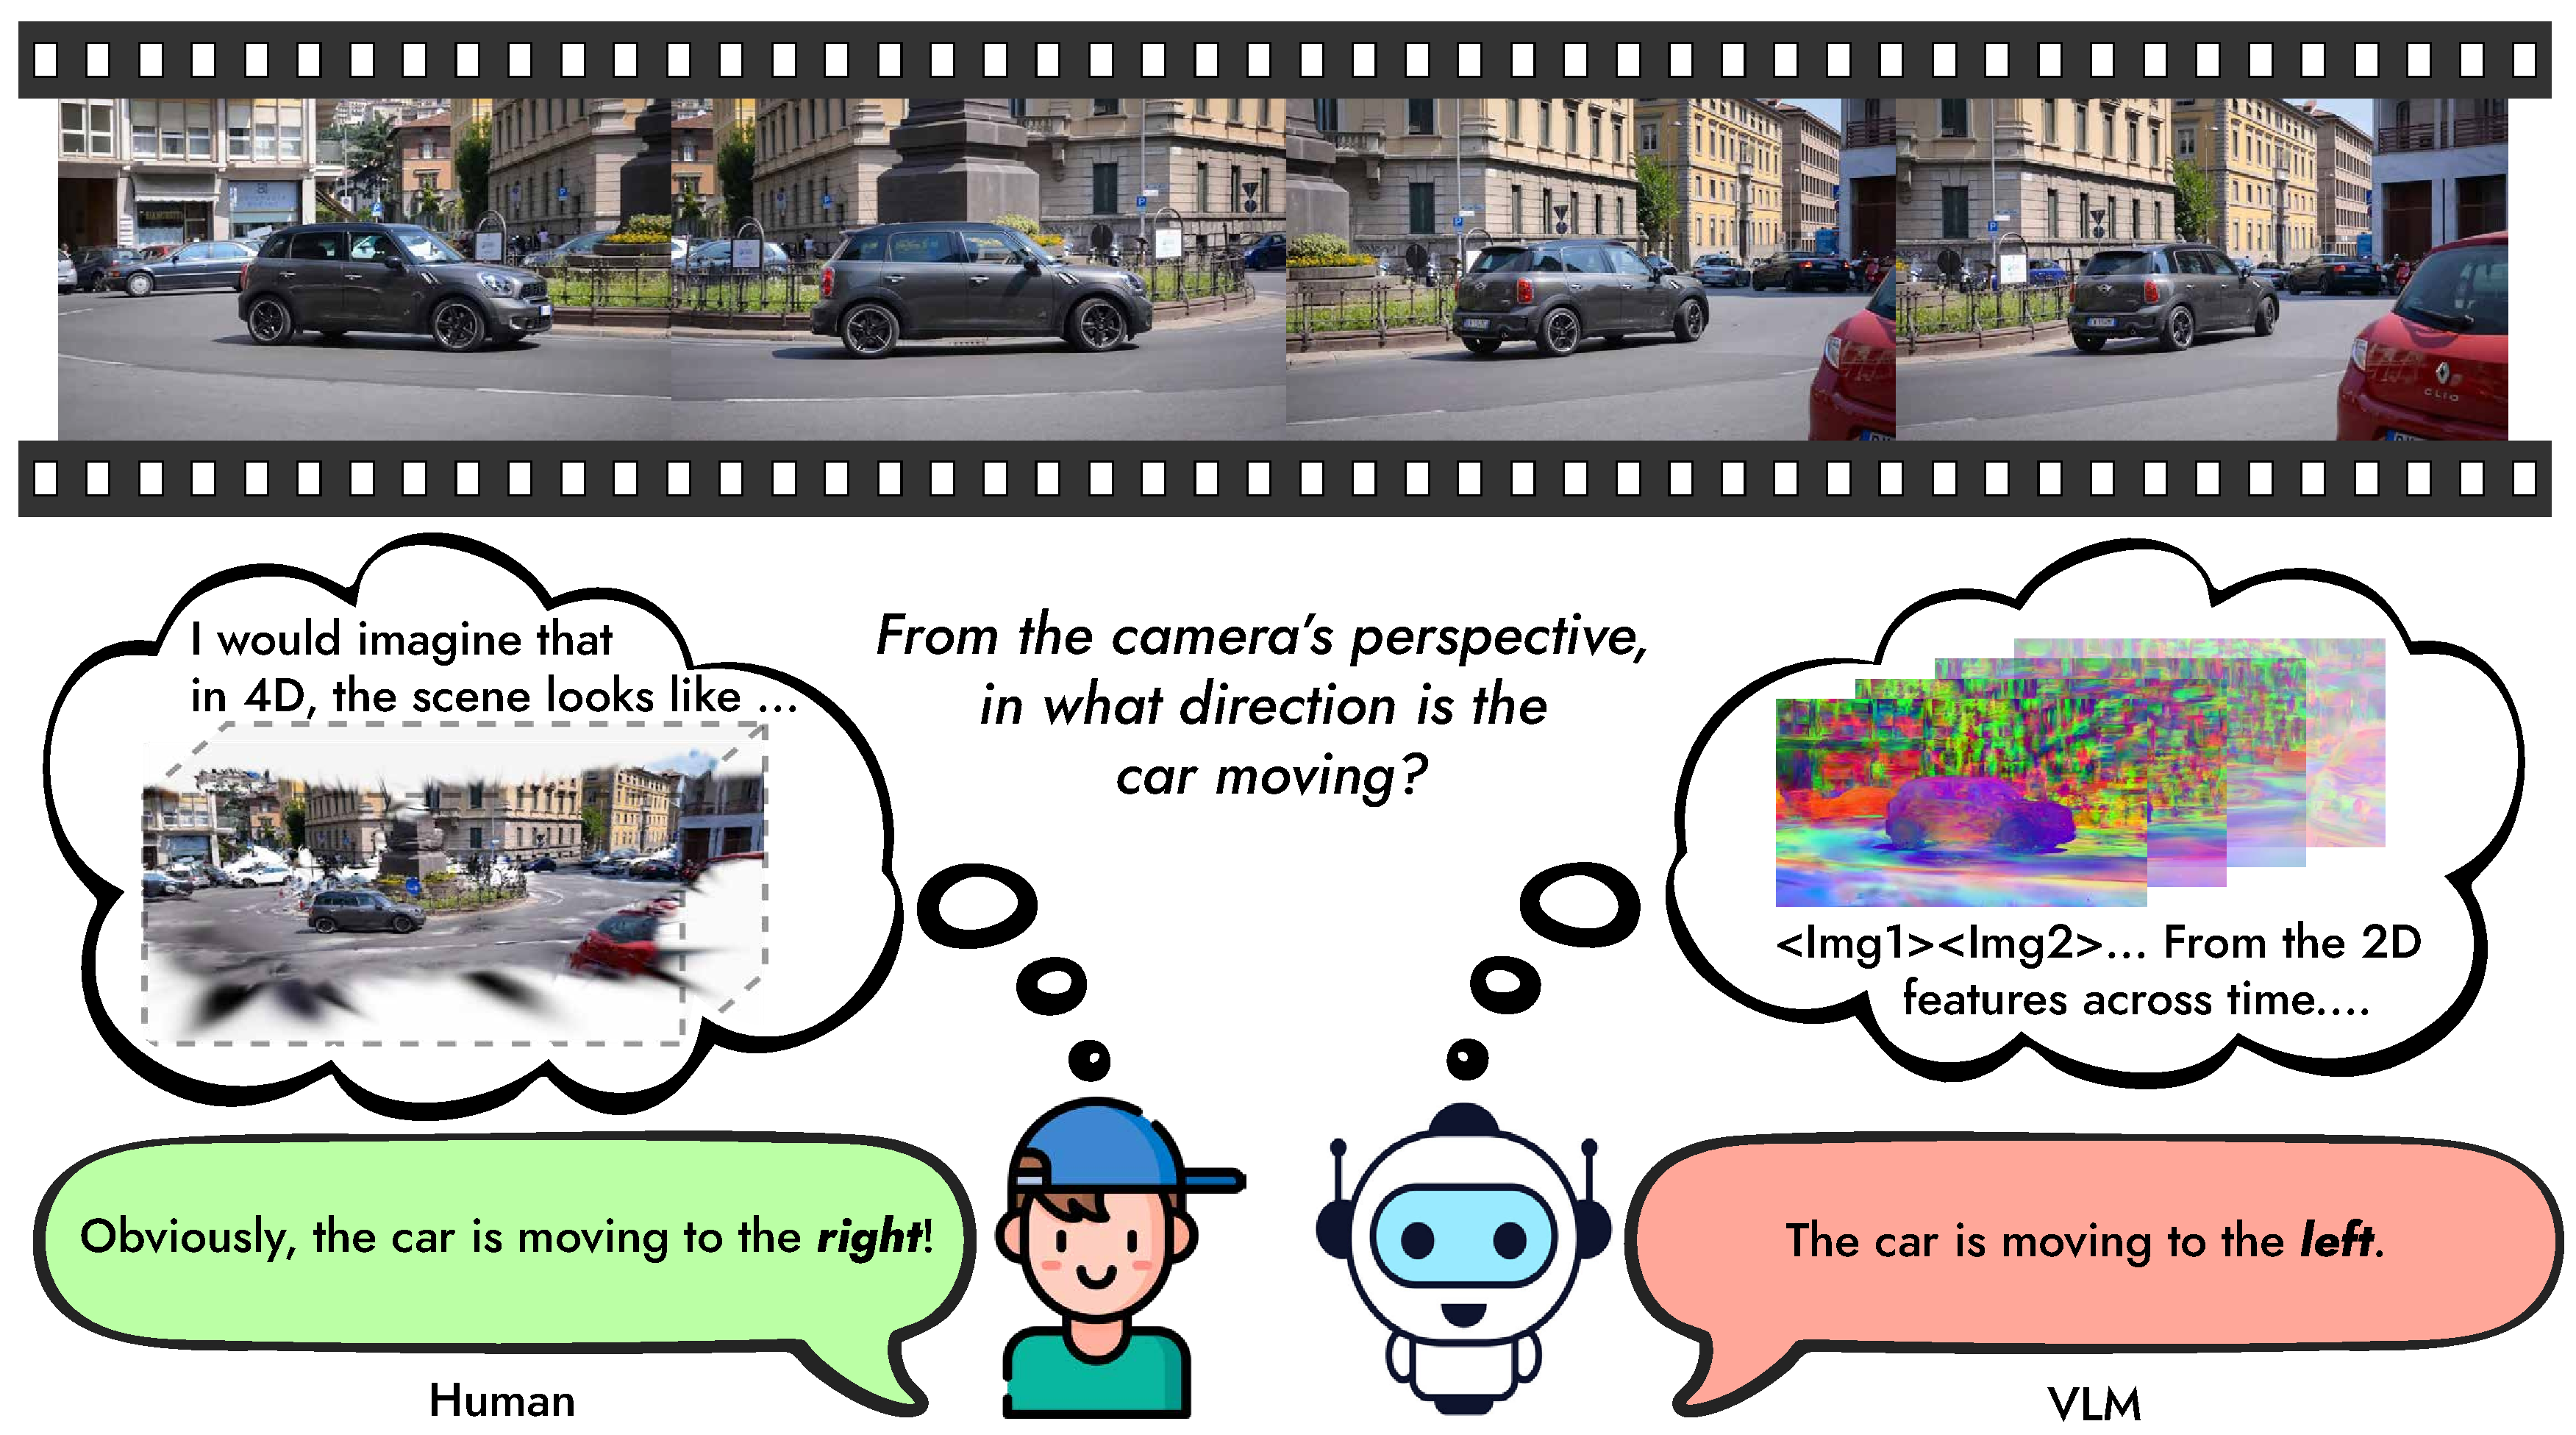
\includegraphics[width=\textwidth]{figures/teaser_v5.pdf} %\vspace{-2mm}
    \vspace{-5mm}
    \hfill\caption{\textbf{Spatiotemporal (4D) Awareness}. Humans intuitively reason in 4D (3D space + time), effortlessly reconstructing the dynamic spatial trajectory of moving objects from any perspective. In contrast, current Vision Language Models (VLMs) typically rely on aggregating 2D visual features across time, leading to incorrect predictions when motion interpretation requires deeper spatiotemporal reasoning. In this example, humans correctly perceive the car moving to the right, while the VLM (GPT-4o) inaccurately predicts leftward movement.}
    \label{fig:teaser}
    \hfill \vspace{0mm}
    %\captionof{figure}{Test caption}
}]
% \begin{figure}[ht]
%     \centering
%     % Replace 'example-image' with your image file name (e.g., 'myfigure.png')
%     \includegraphics[width=0.5\textwidth]{example-image}
%     \caption{Video Example+SpatioTemporal Question with the answers of 5 of the top video LLMs}
%     \label{fig:myfigure}
% \end{figure}

\begin{abstract}
Vision-language models (VLMs) have shown remarkable capabilities in integrating linguistic and visual reasoning but remain fundamentally limited in understanding dynamic spatiotemporal interactions. Humans effortlessly track and reason about object movements, rotations, and perspective shifts—abilities essential for robust dynamic real-world understanding yet notably lacking in current VLMs. In this paper, we introduce \texttt{VLM4D}, the first benchmark specifically designed to evaluate the spatiotemporal reasoning capabilities of VLMs. Our benchmark comprises diverse real-world and synthetic videos accompanied by carefully curated question-answer pairs emphasizing translational and rotational motions, perspective awareness, and motion continuity. Through comprehensive evaluations of state-of-the-art open and closed-source VLMs, we identify significant performance gaps compared to human baselines, highlighting fundamental deficiencies in existing models. Extensive analysis reveals that VLMs struggle particularly with integrating multiple visual cues and maintaining temporal coherence. We further explore promising directions, such as leveraging 4D feature field reconstruction and targeted spatiotemporal supervised fine-tuning, demonstrating their effectiveness in enhancing spatiotemporal comprehension. Our work aims to encourage deeper exploration into improving VLMs’ spatial and temporal grounding, paving the way towards more capable and reliable visual intelligence for dynamic environments.
\end{abstract}  
\section{Introduction}
\label{sec:intro}
Humans posses an innate ability to perceive, track and interpret motion, spatial and temporal changes, ~\cite{DeFreitas2016Tracking, Marr1981Directional} enable rich interpretations of complex dynamic events from both egocentric and allocentric perspectives \cite{Burgess2006Spatial}. When observing an object move, we can inherently process any changes such as lateral shifts, rotational directions and periodic or repeated actions unfolding along a specific trajectory \cite{Burgess2006Spatial}. These sophisticated perceptual abilities are a product of our spatiotemporal cognition~\cite{Freyd1984Representational}, and form an essential foundation that allows us to comprehend and reason about physical phenomena, object interactions and causal relationships within our environment. ~\cite{Leslie1984Spatiotemporal, Johansson1973Visual}

Vision-language models (VLMs), which can also potentially perceive the motions and spatialtemporal changes in videos, constitute a prominent class of methods designed to emulate or surpass human capabilities in integrated visual and linguistic reasoning~\cite{LeCun1989Backpropagation, Dosovitskiy2021An}. While prior work has focused on static visual understanding from mass training corpuses of language and visual data~\cite{Radford2021Learning} or understanding video such as captioning~\cite{Lu2019ViLBERTPT} and scene understanding~\cite{Chen_2022_CVPR}, we find that the exceptional performance in the prior mentioned tasks does not innately carry over to spatiotemporal capabilities. This limitation is notable given that contemporary state-of-the-art VLMs are typically trained on datasets comprising of billions of annotated video-text pairs~\cite{liu2023world}. In contrast, human infants naturally develop robust spatiotemporal cognition within the first few months of life~\cite{Spelke2007Core}. Another key challenge that inhibits VLM performance in spatiotemporal tasks is the necessity to implicitly or explicitly reconstruct a four-dimensional (4D) representation of dynamic scenes and subsequently reason over such reconstruction~\cite{wang2024compositional}. As illustrated in \cref{fig:teaser}, the car is advancing forwards and turning to the left in its own frame of reference. However, from the camera's perspective, its motion appears as a combination of heading to the right and receding into the distance despite the car being in the center of the frame due to camera view rotation. Human observers can seamlessly disentangle these complex dynamics, accurately interpreting trajectories by synthesizing diverse visual cues including camera rotation compensation, stationary scene landmarks, prior knowledge of 3D and 4D environmental structures, and perspective projections \cite{Marr1981Directional,Burgess2006Spatial,Leslie1984Spatiotemporal,Freyd1984Representational}. The inability of current VLMs to similarly integrate these cues underscores an important gap. Furthermore, bridging this gap will require VLMs to develop more sophisticated mechanisms for reconstructing and reasoning over dynamic scenes, potentially drawing on  insights from cognitive science and neuroscience on how humans process and integrate spatial and temporal information.
\begin{figure}[t]
    \centering
    % Replace 'example-image' with your image file name (e.g., 'myfigure.png')
    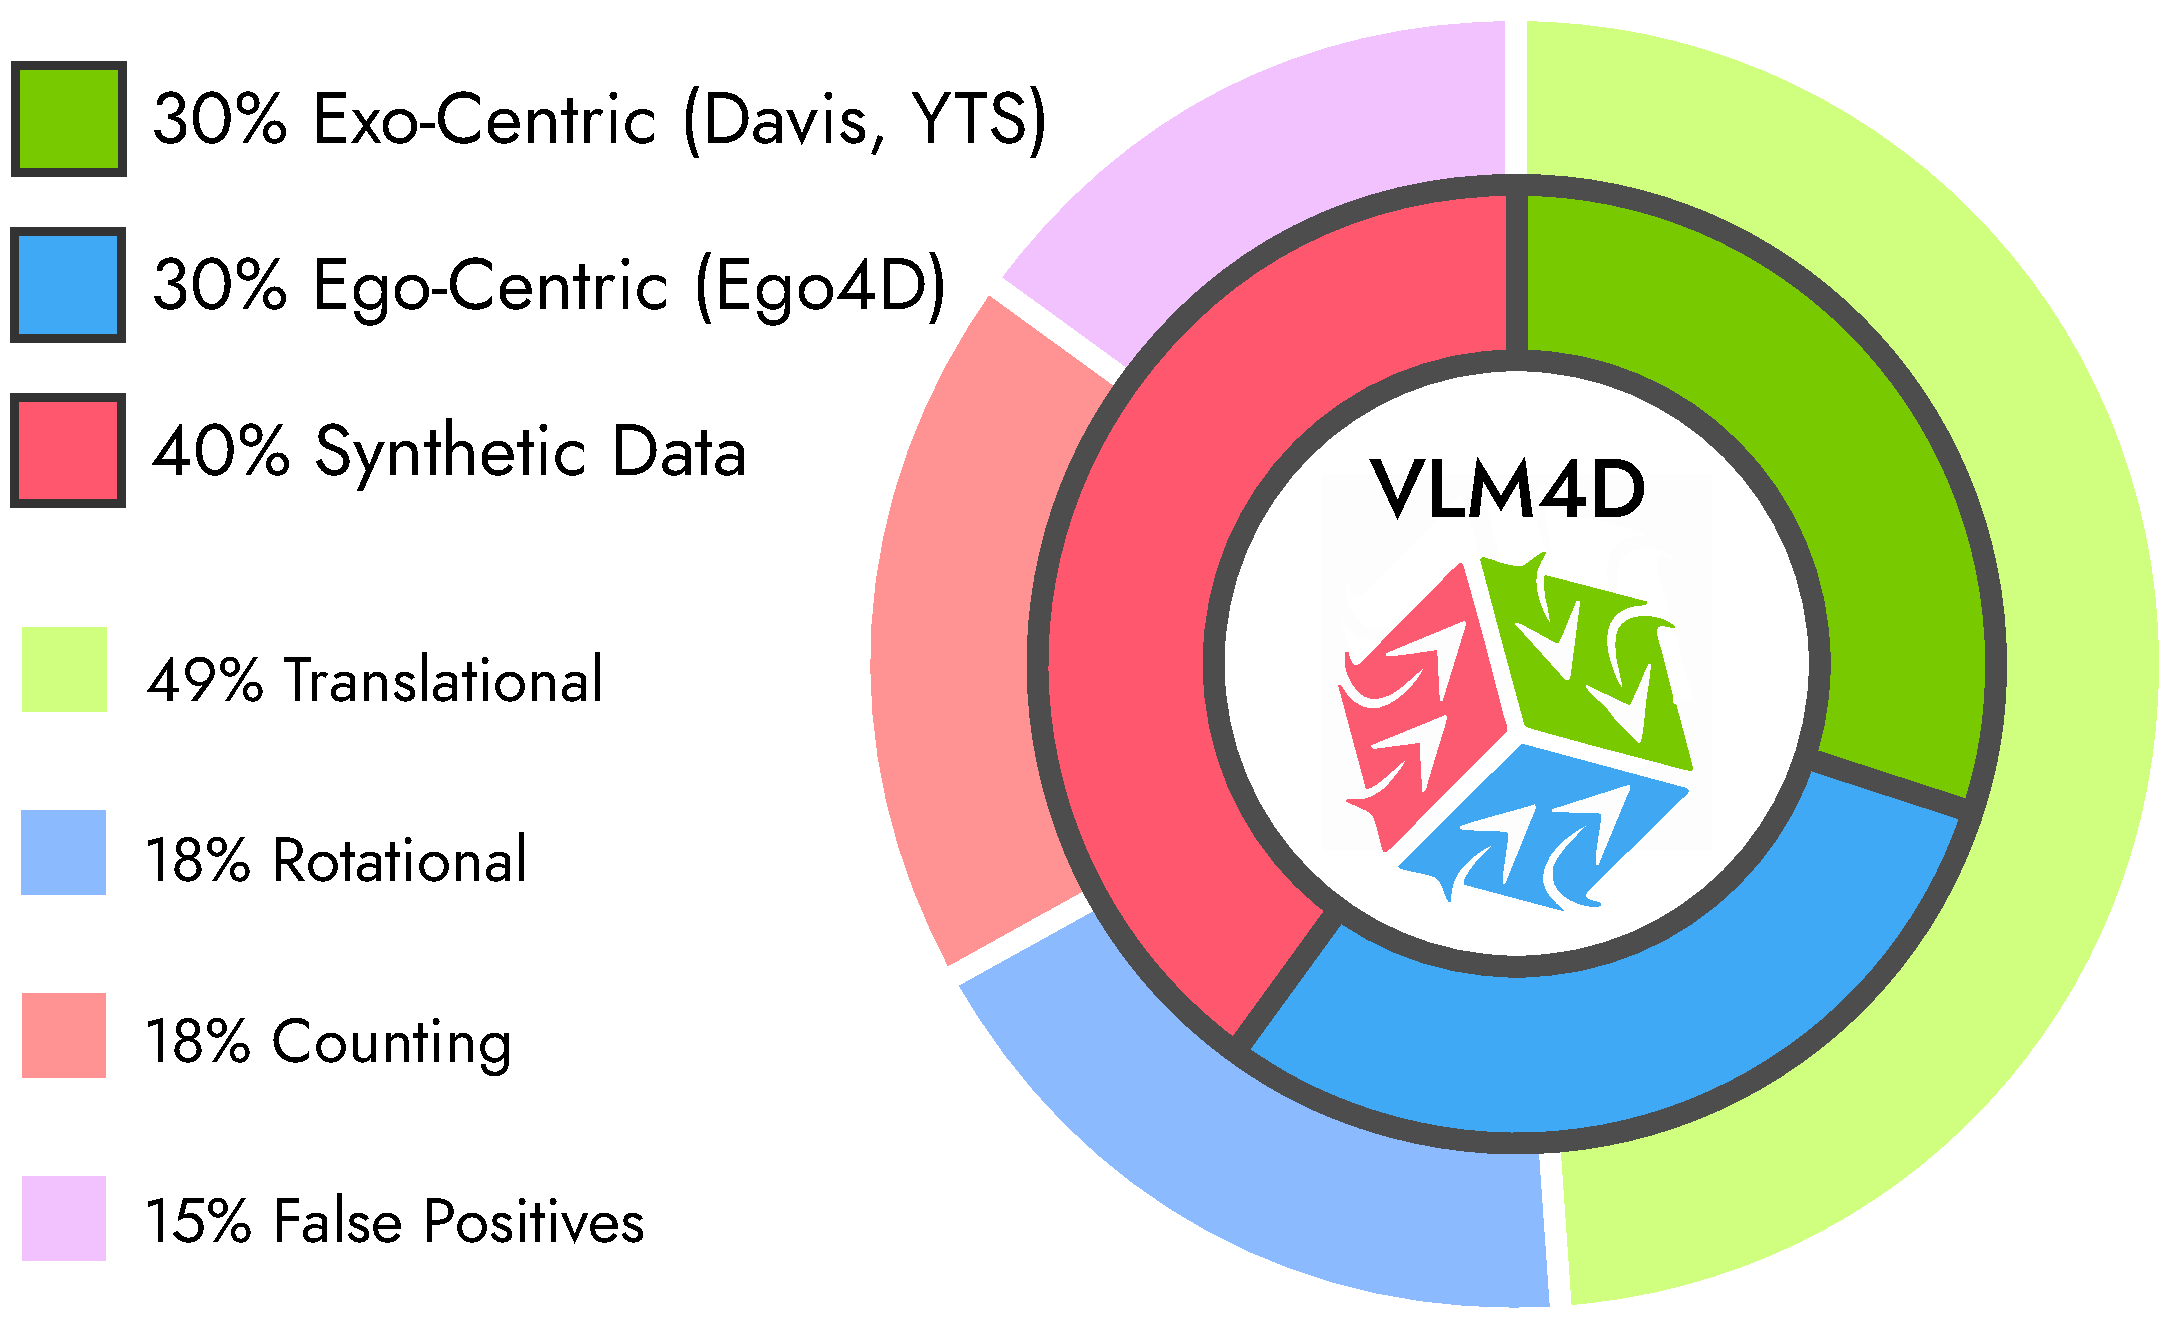
\includegraphics[width=0.45\textwidth]{figures/piechart_dataset_stats.pdf}
    \caption{\textbf{Distribution of Dataset Sources and Annotations.} Breakdown of our dataset illustrating the proportions of data sourced from third-person (Davis, YouTube), first-person (Ego4D), and synthetic data, categorized by annotation types: translational, rotational, action, counting, and false positives.}
    \label{fig:data_piechart}
    \vspace{-0.3cm}
\end{figure}

\begin{figure*}[ht]
    \centering
    % Replace 'example-image' with your image file name (e.g., 'myfigure.png')
    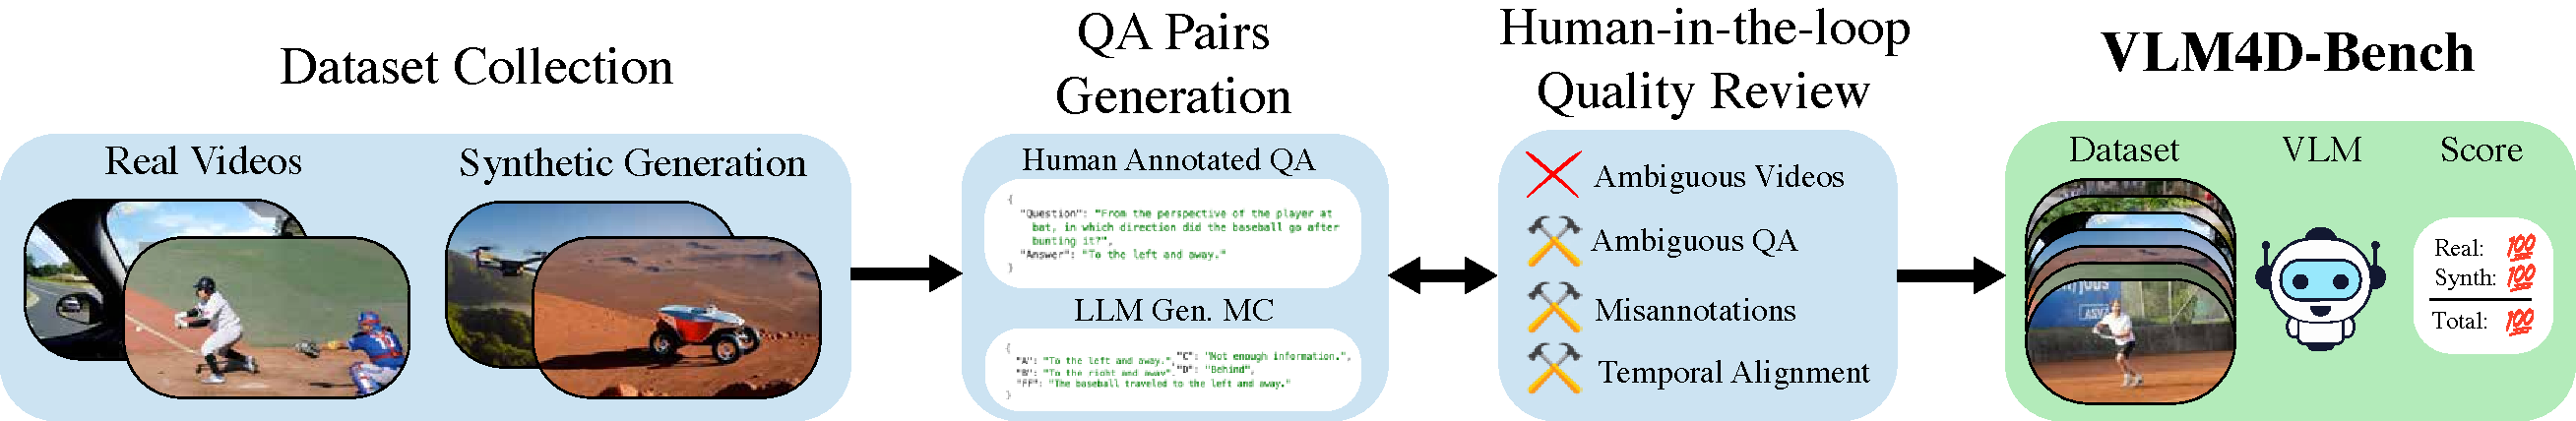
\includegraphics[width=1\textwidth]{figures/dataset_generation_v2.pdf}
    \caption{\textbf{Dataset Generation and Annotation Pipeline.} Our dataset was constructed by collecting real videos and generating synthetic data, followed by human-in-the-loop quality reviews to address ambiguous videos and annotations. After temporal alignment and quality assurance, human-annotated questions and answers were created, complemented by multiple-choice questions generated by large language models (LLMs). The final dataset includes real-world and synthetic video data with comprehensive VLM scoring metrics.}
    \label{fig:dataset_pipeline}
    \vspace{-0.4cm}
\end{figure*}

With the mentioned limitations of exisiting VLMs, to effectively characterize and challenge the existing spatiotemporal reasoning abilities of VLMs, we directly evaluate their capacity to track complex directional movements and perspective transformations over time. We introduce \texttt{VLM4D}, a rigorous benchmark specifically designed to probe the spatiotemporal grounding capabilities of current vision-language models. Through this contribution, we aim to catalyze research that addresses the critical gap in spatiotemporal understanding and reasoning within VLMs and provide a foundational analysis highlighting key deficiencies in existing models. 

We summarize our main~\textbf{contributions} as follows:
\begin{enumerate}
\item We propose the first benchmark~\texttt{VLM4D} explicitly designed to rigorously evaluate the spatiotemporal reasoning capabilities of Vision-Language Models (VLMs).
\item We introduce a novel, meticulously curated dataset consisting of diverse real-world and synthetic video sequences paired with carefully crafted spatiotemporal question-answer (QA) annotations.
\item We conduct an analysis to identify critical limitations in the spatiotemporal reasoning performance of contemporary VLMs, highlighting fundamental challenges and charting clear directions for impactful future research.
\end{enumerate}








\section{Related Work}
\label{sec:related_work}

\paragraph{Spatiotemporal Understanding in Vision Language Models}%
Vision Language Models (VLMs) have evolved rapidly by fully leveraging the significant achievements of Large Language Models (LLMs)~\cite{brown2020language, devlin2019bert, wei2021finetuned, bai2023qwen, touvron2023llama, radford2018improving} and large-scale visual instruction tuning datasets~\cite{liu2023visual, zhu2023minigpt, dai2023instructblip}. While VLMs~\cite{gong2023multimodal, liu2023visual, zhu2023minigpt, abouelenin2025phi4minitechnicalreportcompact, hurst2024gpt, li2024llava, team2024gemini, wang2024qwen2} exhibit transformative potential for applications such as embodied AI~\cite{suglia2024alanavlm, driess2023palm, kim2024openvla}, robotics~\cite{wang2024vlm, patel2025real}, and world modeling~\cite{liu2024world, zhang2024combo}, most existing methods remain constrained to static images, focusing narrowly on spatial understanding while overlooking the dynamic temporal dimension inherent in real-world interactions. To bridge this gap, emerging research~\cite{li2023videochat, zhang2023video, cheng2024videollama, maaz2023video, zhang2025videollama} has begun exploring video modality integration, aiming to equip VLMs with spatial-temporal awareness critical for tasks like video comprehension, where both contextual details and motion dynamics are essential. For example, VideoLLM-MoD~\cite{wu2024videollm} proposes to address the efficiency issue when processing long-term video by mixture-of-depths. ~\cite{yuan2024videorefer} introduces VideoRefer to enhance the finer-level (like object-level) spatial-temporal video understanding of VLMs. Grounded-VideoLLM~\cite{wang2024grounded} also targets for fine-grained video understanding through incorporating an additional temporal stream. In this work, we aim to rigorously evaluate the 4D spatial-temporal reasoning capabilities of state-of-the-art VLMs, probing how and to what extent these models internalize spatial intelligence and temporal dependencies.

\paragraph{VLM Benchmarks}% 
Following the development trends of VLMs, benchmarking VLMs shares the similar trajectory by first evaluating vision QA on static images~\cite{li2024seed, liu2024mmbench, he2024mmworld,yue2024mmmu}, to align with models’ early focus on 2D understanding. As VLMs evolved to tackle dynamic scenarios, benchmarks expanded to evaluate general-purpose video comprehension tasks that probe temporal coherence and event understanding~\cite{ning2023video, khattak2024good, li2024videoeval, fu2024video, li2024mvbench}. Notably, MMVU~\cite{zhao2025mmvu} further proposes a knowledge-intensive benchmark to assess the expert-level reasoning ability of current video-based large models. However, while these works assess perception and semantic understanding, they largely overlook the explicit evaluation of spatial-temporal awareness, a core capability for real-world applications requiring 4D (3D space + time) reasoning. Recent efforts like~\cite{yang2024thinking} pioneer benchmarks for 3D visual-spatial intelligence but restrict evaluation to static 3D scene, neglecting the interplay of object motion and temporal dynamics intrinsic to videos. In this work, we introduce \texttt{VLM4D}, the first benchmark designed to holistically evaluate the 4D intelligence in VLMs, unifying spatial understanding, temporal continuity, and motion reasoning. By curating tasks that demand precise analysis of dynamic interactions (e.g., direction prediction, perspective anticipation, and motion reasoning), \texttt{VLM4D} exposes critical gaps in current models' ability to internalize spatiotemporal relationships. Our work not only advances the granularity of VLM evaluation but also shares insights and potential solutions to improve the model performance.

\begin{figure*}[t]
    \centering
    % Replace 'example-image' with your image file name (e.g., 'myfigure.png')
    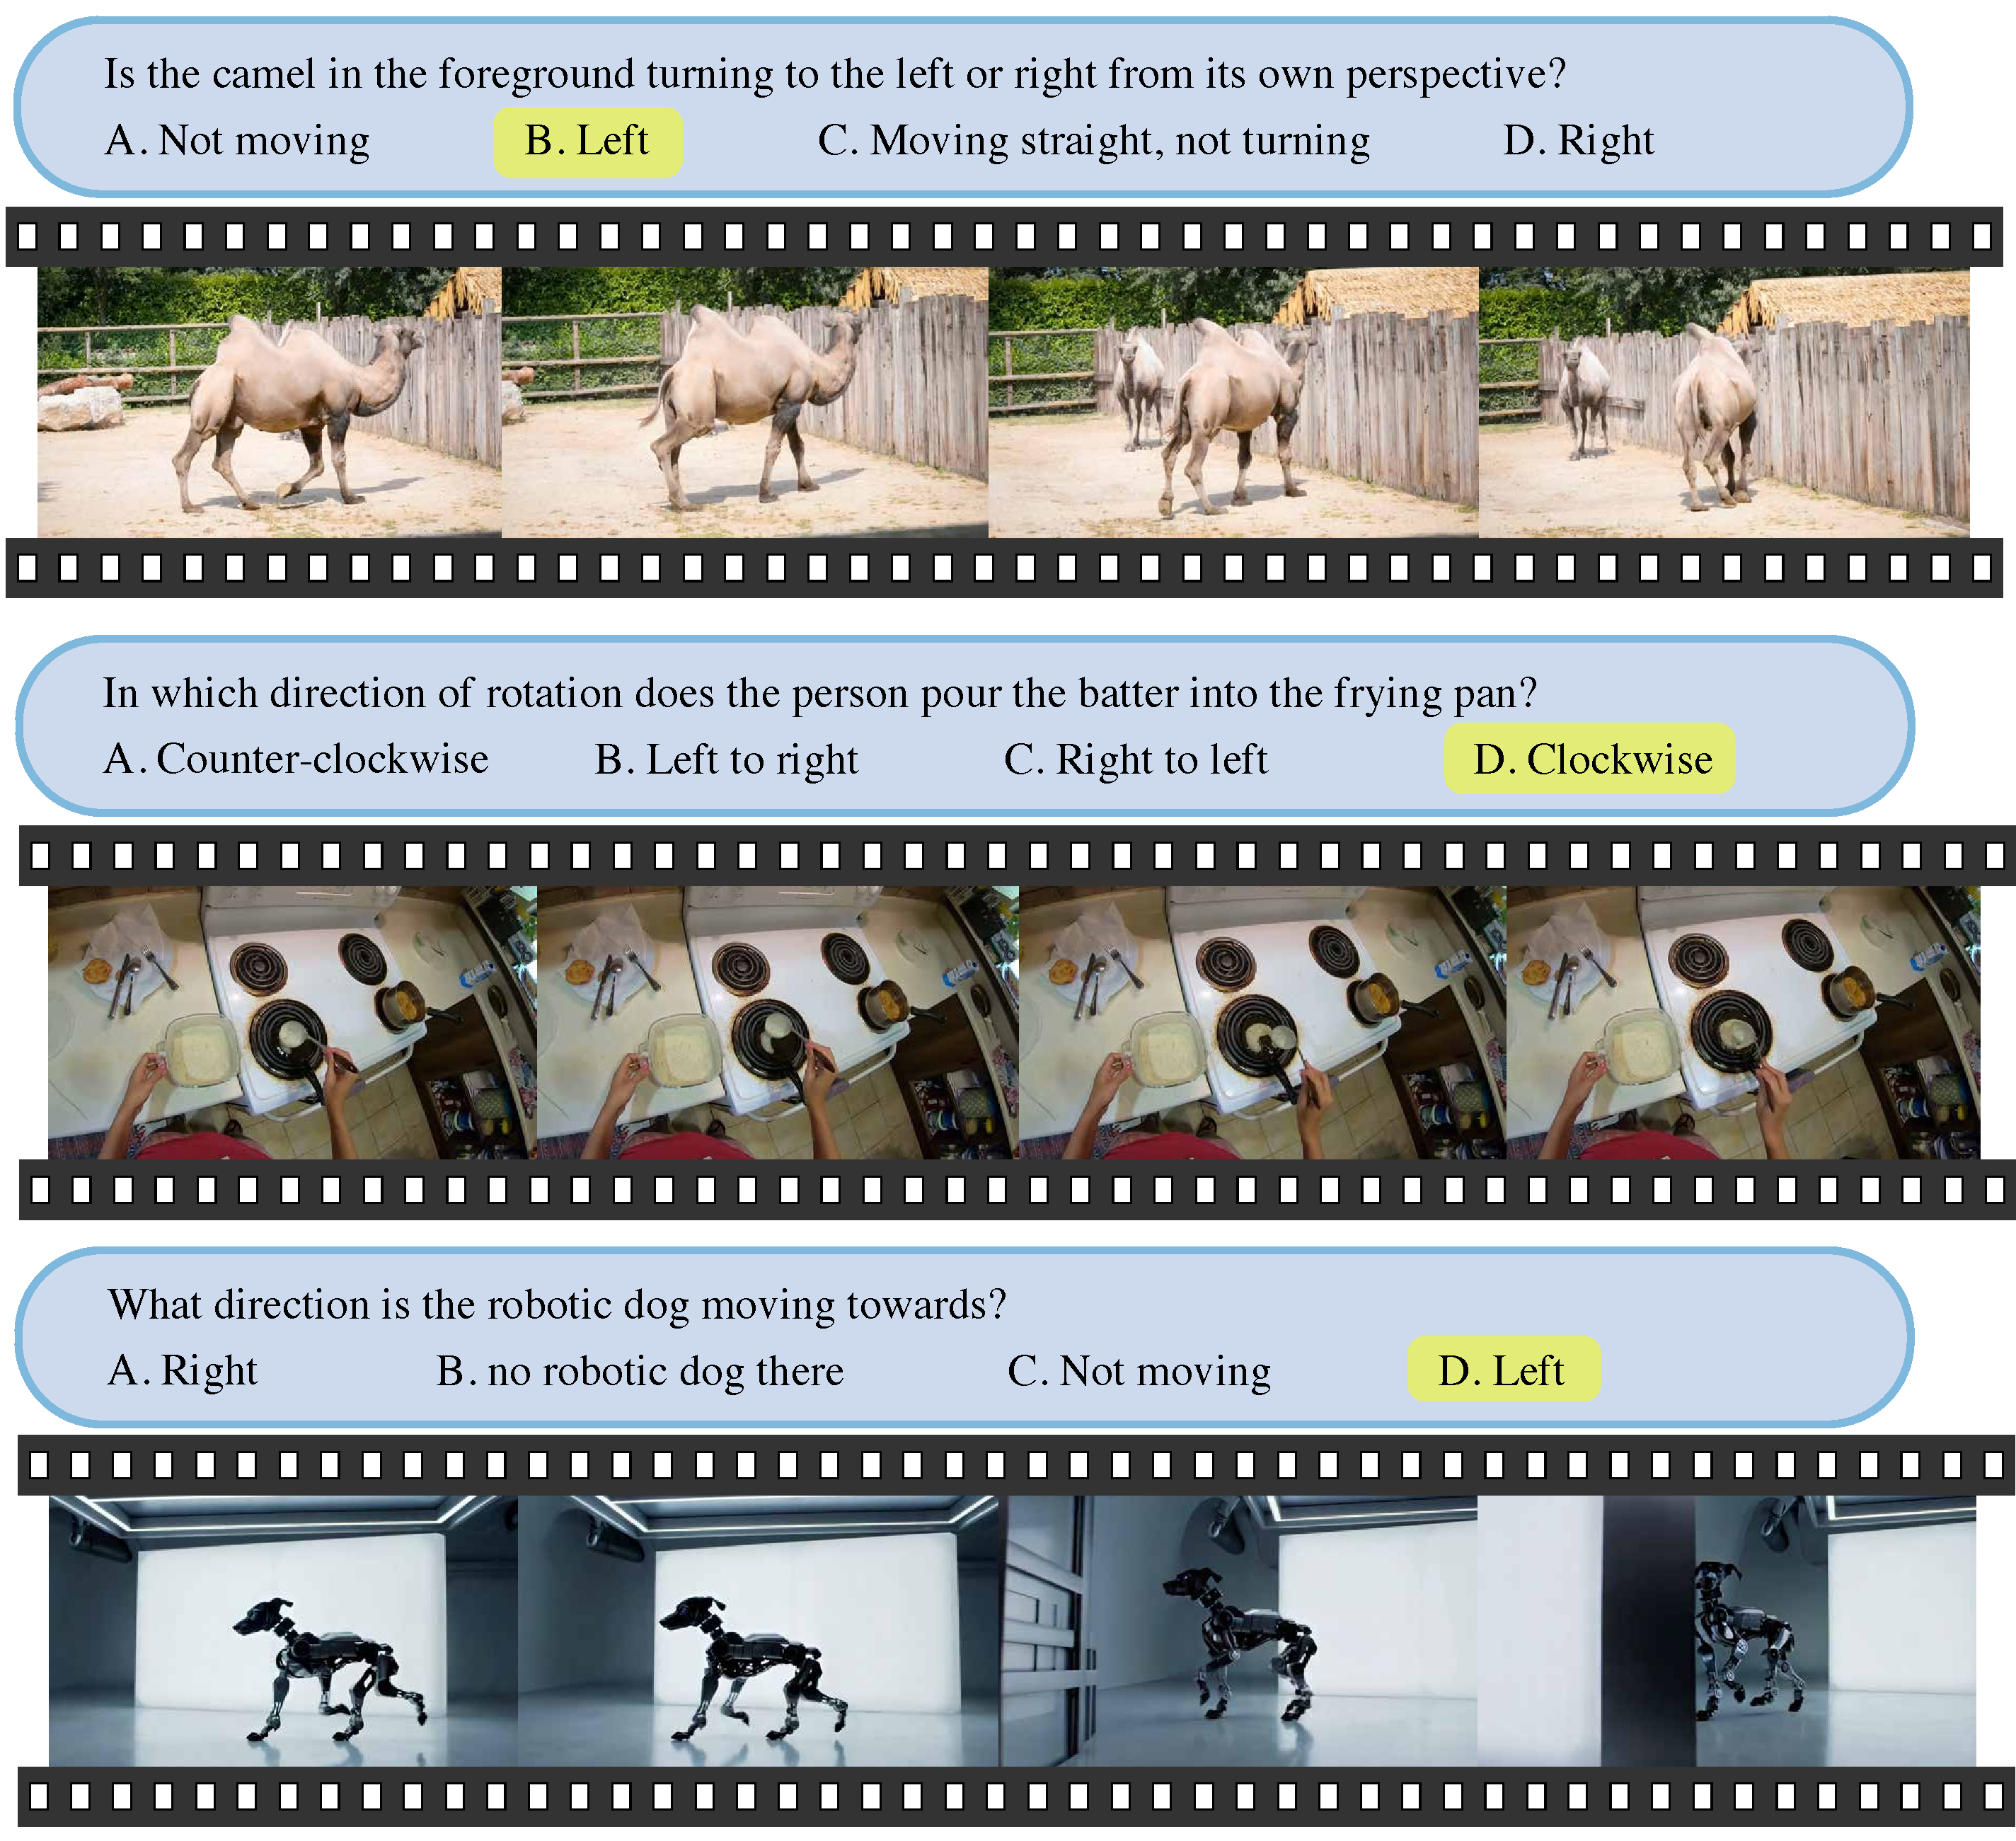
\includegraphics[width=0.8\textwidth]{figures/dataset_qualitative_v3.pdf}
    \caption{\textbf{Qualitative Examples of Dataset Annotations.} (Top) A third-person video with translational annotations (``camel turning left from its perspective"). (Middle) A first-person video with a rotational question (``clockwise rotation of ladle"). (Bottom) A synthetic scene with action recognition ``robotic dog moving right"). }
    \label{fig:qualitative_examples}
    \vspace{-0.5cm}
\end{figure*}
\section{The \texttt{VLM4D} Benchmark}
We introduce \texttt{VLM4D}, the first benchmark specifically designed to test the spatiotemporal reasoning abilities of VLMs. \texttt{VLM4D} consists of 1,000 videos paired with over 2,000 question-answer pairs, each carefully designed to assess both spatial and temporal understanding jointly. The majority of these videos are sourced from datasets with rich spatiotemporal characteristics, thus ensuring a diverse range of motion-related scenarios. We augment the dataset with synthetic videos generated by a world-foundation model, Cosmos~\cite{agarwal2025cosmos}, that has been modified using techniques introduced in~\cite{he2024mojito} to obtain more accurate correspondence between motion-oriented prompts and the resulting generated video. Figure~\ref{fig:data_piechart} illustrates the composition of our dataset.

\subsection{Benchmark Construction}
Unlike prior work that often relies heavily on LLMs and VLMs to generate first iterations of benchmarks and datasets~\cite{chen2024sharegpt4video} followed by human quality control - we found that existing VLMs and automated methods showed significant limitations in terms of realiability and quality. This shortcoming necessitated direct human annotations that were then followed by augmentation by LLMs to ensure a high-quality benchmark. An overview of the benchmark curation pipeline is shown in \cref{fig:dataset_pipeline}. 

\paragraph{Real Video Data Collection} Real-world videos were sourced from datasets with rich spatiotemporal characteristics that ensured diverse motion and perspective variations. For egocentric data, we primarily relied on the Ego4D dataset~\cite{grauman2022ego4d}, while most object-centric data points were collected from the Davis~\cite{davis2017} and YouTube-VOS~\cite{xu2018youtube} datasets. To minimize confounders and to focus attention of VLM abilities to only spatiotemporal reasoning, we preprocessed the videos by temporally segmenting and centering them around the most relevant action thus resulting in videos with an average duration of $5$-$15$ seconds. This ensures that the key event described in the question is clear and reduces ambiguities or confounders that would reduce VLM accuracy. 

\paragraph{Synthetic Video Generation}  
For synthetic video generation, we use Cosmos~\cite{agarwal2025cosmos} as our video generation backbone. To ensure that the generated videos align with the intended object moving directions, we incorporate input bounding boxes as additional spatial guidance. Specifically, we follow the approach introduced in~\cite{he2024mojito} modifying the diffusion forward steps to enforce object localization constraints at each timestep, ensuring consistency between the generated object direction and the user-specified trajectory. The average duration of generated synthetic videos is $5$ seconds. To maintain high-quality outputs, we perform a manual verification step after generation, filtering out low-quality videos and retaining only those that accurately match the specified directions. Once a video is generated, we use an LLM (GPT-4o) to generate two types of questions for evaluation: Direct questions, which are derived directly from the textual prompt used to generate the video; Counterfactual questions, which involve querying about non-existent objects in the generated scene. Both question types follow the format: ``What direction is the $\langle$Object Name$\rangle$ moving?", where the model must select one of four possible answers: ``left", ``right", ``not moving", or ``no $\langle$Object Name$\rangle$ there." 


\paragraph{QA Generation and Quality Control} Question-answer pairs are primarily constructed through human annotations. The question answer pairs are then supplemented with alternative answers by an LLM (GPT-4o) for multiple choice (MC) questions. To ensure high-quality annotations, a rigorous human verification process was applied where ambiguous videos were filtered out and vague, misleading, or incorrect QA pairs were refined to allow for spatial and temporal alignment between the language and visual content. Figure~\ref{fig:qualitative_examples} showcases some qualitative examples of annotations for different types of videos.

\paragraph{Assessing Human Performance}
To establish a human performance baseline on our benchmark, we conducted an evaluation in which participants independently answered 100 randomly sampled questions from the dataset. The accuracy of human responses was then aggregated to approximate the performance of human spatiotemporal reasoning on thedataset. 

\subsection{Categorizing Spatiotemporal Performance}
To systematically evaluate spatiotemporal reasoning capabilities, we first categorize videos into two primary groups: egocentric (first-person) videos and exocentric (third-person) videos. Egocentric videos are sourced from the Ego-4D~\cite{grauman2022ego4d} dataset where scenes are captured from a head-mounted camera, thus offering dynamic video data that is inherently coupled with the individual's actions. Exocentric videos encompass a diverse range of recorded scenes, from sports footage to everyday scenes. Beyond this categorization, we also evaluate spatiotemporal performance across four dimensions: translational movement (TM), rotational movement (RM), spatiotemporal counting (STM), and false positives (FP). Translational movement assesses a model's ability to track linear motion within scenes, while rotation movement evaluates the understanding of changes in orientation and perspective shifts over time. Spatiotemporal counting extends these core motion-based tasks by requiring a more complex reasoning strategy to determine the number objects performing a translation or rotational movement. Lastly, the false positives category measures the model's reliability in recognizing whether any motion took place. By structuring the benchmark along these axes, we aim for a comprehensive framework for assessing spatiotemporal reasoning (Figure~\ref{fig:radar_plot}).

\begin{table*}[h]
    \centering
    \resizebox{1.0\linewidth}{!}{
    \renewcommand{\arraystretch}{1.2}
    \arrayrulecolor{black} % Ensures solid borders remain black
    % \begin{tabular}{l l l c c c c c}
    \begin{tabular}{l l l c c c c c c c}
    \toprule
    \textbf{Organization} & \textbf{Model} & \textbf{Release} & \multicolumn{3}{c}{\textbf{Real}} & \multicolumn{3}{c}{\textbf{Synthetic}} & \textbf{Overall} \\
    \cmidrule(lr){4-6}
    \cmidrule(lr){7-9}
    & & & \textbf{Ego-centric} & \textbf{Exo-centric} & \textbf{Average} & \textbf{Directional} & \textbf{FP} & \textbf{Average} \\
    \midrule
         % \rowcolor[HTML]{e1f0f5}\multicolumn{8}{l}{\textbf{Baselines}} \\
         % \midrule
         User Study & Human Performance &  & 99.6 & 99.7 & 99.7 & 91.8 & 100 & 95.9  & 98.3     \\
         Random & Random Selection  &  & 24.4 & 23.2 & 23.6 & 25.5 & 24.7 & 25.1 & 24.2    \\

        \midrule
        \rowcolor[HTML]{e1f0f5}\multicolumn{10}{l}{\textbf{Latest Proprietary VLMs}} \\
        \midrule
        OpenAI & GPT-4o & 2024-11 & \cellcolor[HTML]{FFB366}{\textbf{54.3}} & \cellcolor[HTML]{FFB366}{\textbf{61.2}} & \cellcolor[HTML]{FFB366}{\textbf{58.9}} & \cellcolor[HTML]{FFE5CC}{47.8} & 43.0 & 45.4 & \cellcolor[HTML]{FFCC99}{53.9} \\
        \arrayrulecolor{lightgray} \hdashline
        Google & Gemini 2.0 Pro & 2025-2 & 44.8 & \cellcolor[HTML]{FFE5CC}{50.5} & 48.7 & 42.8 & 41.8 & 42.3  & 46.3     \\
        \hdashline
        xAI & Grok-2-Vision & 2024-12 & 44.1 & 48.8 & 47.3 & \cellcolor[HTML]{FFCC99}{49.0} & 60.5 & \cellcolor[HTML]{FFE5CC}{54.8} & \cellcolor[HTML]{FFE5CC}{50.0} \\
        \arrayrulecolor{black} \midrule
        \rowcolor[HTML]{e1f0f5}\multicolumn{10}{l}{\textbf{Open-source Image VLMs}} \\
        \midrule
        Meta & Llama-3.2-11B-Vision & 2024-9 & 35.2 & 36.1 & 35.8 & 38.3 & 55.8 & 47.0 & 39.9   \\
        \arrayrulecolor{lightgray} \hdashline
        Microsoft & Phi-3.5-Vision & 2024-7 &  36.3 & 39.1 & 38.2 & 26.5 & 37.5 & 32.0 & 35.9 \\
        \arrayrulecolor{lightgray} \hdashline
        DeepSeek &  DeepSeek-VL2-Tiny & 2024-12 &  31.4 & 32.5 & 32.2 & 42.8 & 25.5 & 34.1 & 32.9 \\
        % & DeepSeek-VL2 & 2024-8 &  - & - & - & - & -  \\
        % & DeepSeek-VL2-Small & 2024-8 &  - & - & - & - & - \\
        \arrayrulecolor{lightgray} \hdashline
        Shanghai AI Lab & InternVL2.5-38B & 2024-11 & 42.8  & \cellcolor[HTML]{FFCC99}{53.2} & \cellcolor[HTML]{FFE5CC}{49.7} & 37.5 & 55.5 & 46.5 & 48.6\\
        & InternVL2.5-8B & 2024-11 & 40.8 & 41.1 & 41.0 & 40.8 & 47.0 & 43.9 & 42.1   \\
        & InternVL2-8B & 2024-6 & 33.2 & 38.2 & 36.5 & 34.8 & 58.0 & 46.4 & 40.2  \\
        \arrayrulecolor{lightgray} \hdashline
        Mistral AI & Pixtral-12B & 2024-9 & 36.3 & 32.9 & 34.0 & 41.0 & 17.3 & 29.1 & 32.2  \\
        \arrayrulecolor{lightgray} \hdashline
        Rhymes & Aria & 2024-11 &  42.3 & 44.0 & 43.5 & 35.3 & 56.3 & 45.8 & 44.3  \\
        \arrayrulecolor{lightgray} \hdashline
        HuggingFaceM4 & Idefics3-8B & 2024-8 & 34.3 & 36.2 & 35.6 & 33.5 & 47.3 & 40.4 & 37.4  \\
        \arrayrulecolor{lightgray} \hdashline
        H2O & H2OVL-Mississippi-2B & 2024-10 &  37.0 & 33.3 & 34.5 & 27.3 & 41.0 & 34.1 & 34.4  \\
        \arrayrulecolor{black} \midrule
        \rowcolor[HTML]{e1f0f5} \multicolumn{10}{l}{\textbf{Open-source Video VLMs}} \\
        \midrule
        Alibaba & Qwen2.5-VL-7B & 2025-1 & 42.3 & 45.0 & 44.1 & 39.3 & 48.5 & 43.9 & 44.0   \\
        & Qwen2.5-VL-72B-AWQ & 2025-1 & \cellcolor[HTML]{FFE5CC}{49.9} & 48.7 & 49.1 & \cellcolor[HTML]{FFB366}{\textbf{54.3}} & \cellcolor[HTML]{FFB366}{\textbf{72.8}} & \cellcolor[HTML]{FFB366}{\textbf{63.5}} & \cellcolor[HTML]{FFB366}{\textbf{54.4}}  \\
        & Qwen2-VL-7B & 2024-8 & 36.1 & 38.2 & 37.5 & 38.5 & 40.3 & 39.4 & 38.2 \\
        & Qwen2-VL-72B-AWQ & 2024-9 & 43.0 & 46.2 & 45.2 & 43.8 & \cellcolor[HTML]{FFCC99}{71.0} & \cellcolor[HTML]{FFCC99}{57.4} & 49.7 \\
        \hdashline
        DAMO & VideoLLama3-2B & 2025-1 & 48.6 & 43.7 & 45.3 & 29.0 & \cellcolor[HTML]{FFE5CC}{69.8} & 49.4 & 46.8 \\
        & VideoLLama3-7B & 2025-1 & 47.4 & 45.0 & 45.8 & 39.5 & 58.8 & 49.1 & 47.0 \\
        & VideoLLama2.1-7B & 2024-10 & 43.0 & 36.0 & 38.2 & 31.5 & 40.0 & 35.8 & 37.3 \\
        & VideoLLama2-7B & 2024-6 & 36.3 & 16.5 & 23.0 & 25.8 & 45.5 & 35.6 & 27.6 \\
        \hdashline
        OpenGVLab & InternVideo2.5-8B & 2025-1 &  \cellcolor[HTML]{FFCC99}{52.8} & 50.1 & \cellcolor[HTML]{FFCC99}{51.0} & 45.3 & 30.0 & 37.6  & 46.1 \\
        & InternVideo2-8B & 2024-8 & 37.2 & 37.9 & 37.6 & 40.5 & 2.8 & 21.6 & 31.7\\
        \hdashline
        LLaVA & LLaVA-One-Vision-7B & 2024-9 & 32.5 & 33.1 & 32.9 & 32.8 & 36.0 & 34.4 & 33.5  \\
        & LLaVA-NeXT-Video-7B & 2024-6 & 30.3 & 30.9 & 30.7 & 24.5 & 27.3 & 25.9 & 28.9  \\
        & LLaVA-NeXT-Video-34B & 2024-6 & 37.2 & 34.9 & 35.7 & 31.5 & 56.3 & 43.9 & 38.7  \\
        \arrayrulecolor{black} \bottomrule
    \end{tabular}
    }
    \caption{\textbf{Evaluation on \texttt{VLM4D} Benchmark} across various proprietary and open-source VLMs. Top three performers in each category are highlighted from \colorbox[HTML]{FFB366}{dark} (highest) to \colorbox[HTML]{FFE5CC}{light} (third highest). Human and random selection baselines are included for reference.}
\label{tab:result}
\end{table*}  

\section{Evaluation of \texttt{VLM4D} Benchmark}


\subsection{Evaluation Setup}
\paragraph{Benchmark Models}
We evaluate over 10 of the most recently released VLMs thus covering a wide range of model sizes, architectures, and training methodologies. For open-source models, we include Llama-3.2-Vision~\cite{grattafiori2024llama}, DeepSeek-VL~\cite{lu2024deepseek}, InternVL2.5~\cite{chen2024expanding}, Pixtral~\cite{agrawal2024pixtral}, Aria~\cite{li2024aria}, Idefics~\cite{laurenccon2023obelics}, H2OVL~\cite{galib2024h2ovl}, Qwen2-VL~\cite{wang2024qwen2}, Qwen2.5-VL~\cite{yang2024qwen2}, VideoLLama2~\cite{cheng2024videollama}, VideoLLama3~\cite{zhang2025videollama}, Llava-One-Vision~\cite{li2024llava}, Llava-NeXT-Video~\cite{zhang2024llavanextvideo}, InternVideo2~\cite{wang2024internvideo2}, and InternVideo 2.5~\cite{wang2025internvideo2}. When available, we evaluate different parameter sizes for each model type, resulting overall in models ranging from 2 to 72 billion parameters. For closed-source VLMs, we evaluate GPT-4o~\cite{gpt4o}, Gemini 2.0 Pro~\cite{team2024gemini}, and Grok-2-Vision. 

\paragraph{Evaluation Settings}
The evaluations were performed in a zero-shot setting with the video or a set of sampled frames from the video followed by the prompt forming the input. For each model, we evaluate on two different inference settings. In the first setting, the model is directed to output the answer immediately without any reasoning (DO) and in the second evaluation setting, the model is directed to create intermediate reasoning steps, Chain of Thought (CoT)~\cite{wei2022chain}, before inferring the final answer. Additional details about the evaluation setup and prompts are provided in the Appendix.

\paragraph{Metrics} Following prior work~\cite{yang2024thinking} and given the nature of our target task, we use multiple-choice questions for evaluation. The primary metric is accuracy on the multiple choice questions (MCQ). Given the two inference settings mentioned previously, we employ LLM-as-Judge following~\cite{zhao2025mmvu} to grade the VLMs' outputs. LLM-as-Judge was utilized instead of performing string or template matching as we found that especially during CoT, various VLMs may output all possible answers during the reasoning process in varying frequencies and with slight modifications to the format of the possible answer choices in MCQ. Each MCQ contains four possible answers.

\subsection{Benchmark Results}
\paragraph{VLMs Performance} The evaluation results in~\cref{tab:result} reveal several critical insights regarding the spatiotemporal reasoning capabilities of contemporary VLMs on the \texttt{VLM4D} benchmark. First, proprietary VLMs, particularly OpenAI’s GPT-4o, consistently outperform open-source models across nearly all real-world categories, highlighting the performance gap between closed-source and publicly available VLMs. Among open-source models, InternVideo2.5-8B and Qwen2.5-VL-72B-AWQ emerge as notable contenders, with Qwen2.5-VL-72B-AWQ achieving exceptional results on synthetic data, surpassing even GPT-4o. However, all models significantly trail behind human-level performance, emphasizing substantial room for improvement, especially in nuanced spatiotemporal reasoning. These findings underscore a critical gap in current VLM architectures, reinforcing the need for further research into structured 4D scene representations and improved spatiotemporal grounding strategies. We additionally show in ~\cref{fig:radar_plot} for the top-performing models their strengths and weaknesses in the fine-grained categories mentioned in the previous section. As expected, translational motion performs best, followed by rotational motion and spatiotemporal counting. 

\paragraph{Human Level Performance}
We use \textbf{Prolific}, an online platform designed to connect academic researchers with user research participants for human-level performance evaluation. The participants are English-speaking random users verified by this platform without prior knowledge of computer vision. We asked 51 candidates to answer the spatial awareness questions in our benchmark. Each question has four choices, and the user may select only one correct answer. We collect their answers and report the average precision in Table.~\ref{tab:result}



%%%%%%%%%%%%%5



\section{Analysis: Why VLMs Don't Work Well?}

\subsection{Limited Spatiotemporal Cognition}
Despite significant advances in VLMs, their ability to understand and reason about motion, spatial relationships, and temporal coherence remains fundamentally underdeveloped ~\cite{chen2024we, apollo}. Chain of Thought (CoT)~\cite{wei2022chain} is widely employed as a method to improve accuracy through step-by-step reasoning. We showcase a comparison between CoT and DO in ~\cref{fig:cot_vs_do}. Overall, there is no indication of a large advantage of CoT over all evaluated models. Upon deeper exploration of the CoT reasoning of some models, we observe that the reasoning process was primarily flawed in the following ways: irrelevant information and arriving at conclusions that are inconsistent with the reasoning process. Larger models exhibited strategies that would be similar to how a human processes spatiotemporal information, but the resulting execution falls short of human performance. This demonstrates a disconnect between its visual and linguistic knowledge. We provide examples of this behavior in the supplement. 

\begin{figure}
    \centering
    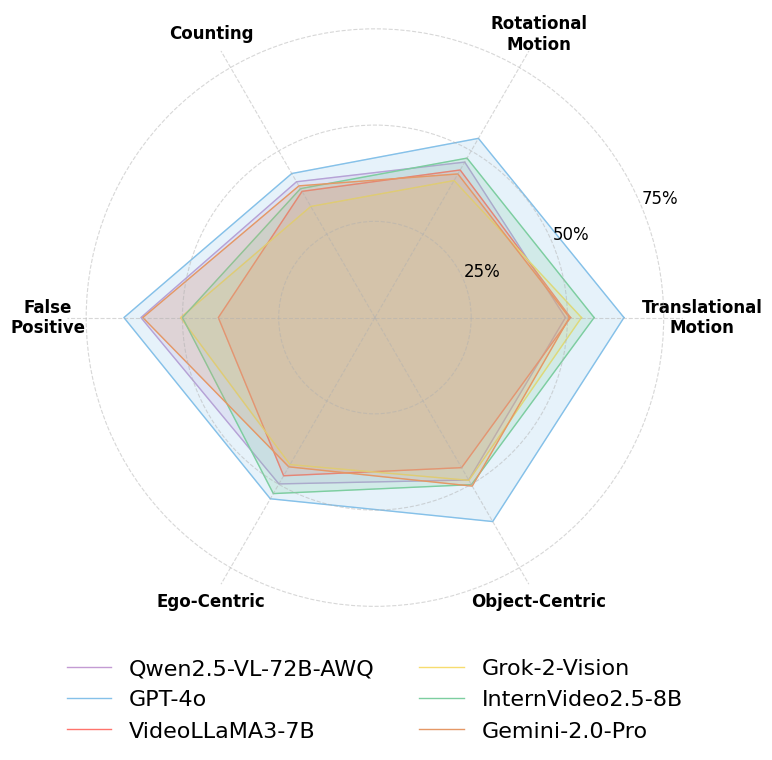
\includegraphics[width=1\linewidth]{figures/radar_plot.png}
    \caption{Model Accuracy Across Real Scene Question Categories of top-performing VLMs.}
    \label{fig:radar_plot}
    \vspace{-0.3cm}
\end{figure}

\begin{figure}
    \centering
    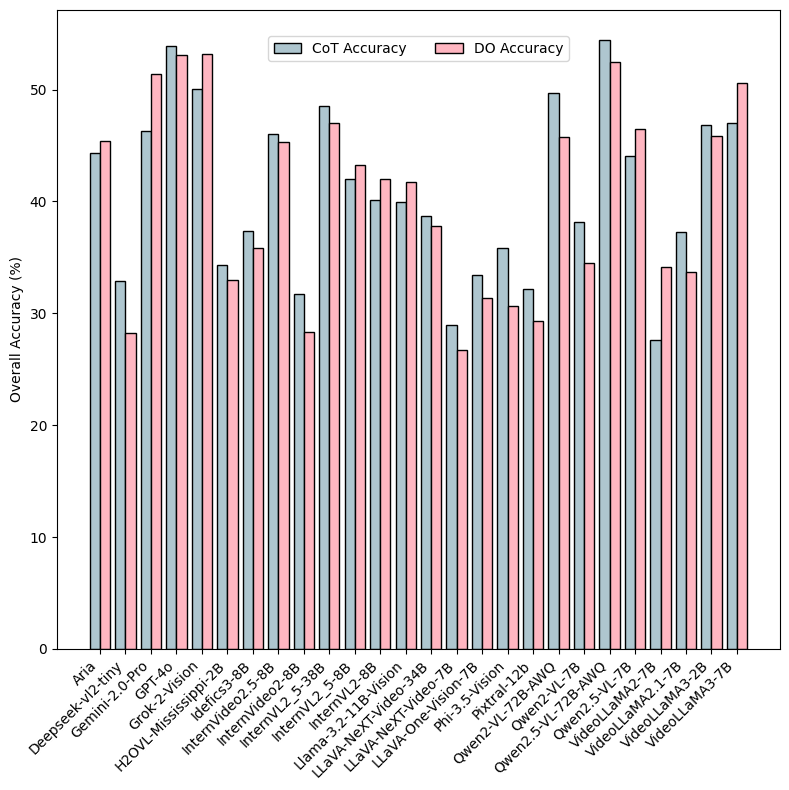
\includegraphics[width=\linewidth]{figures/cot_vs_do.png}
    \caption{\textbf{Comparison of CoT and DO Accuracy Across Models.} Accuracy comparison between Chain-of-Thought (CoT) and Direct Output (DO) prompting across VLMs.}
    \label{fig:cot_vs_do}
    \vspace{-0.5cm}
\end{figure}

\subsection{Deficiencies in Spatiotemporal Labeling}
Another avenue of exploration we undertook is to understand the richness of spatiotemporal labels in popular SFT VLM datasets. Typically, video captioning occurs at the 'scene' level, lacking fine-grained temporal, spatial, and object-level details. We performed an extensive analysis, encompassing over 2 million samples~\cite{chen2024sharegpt4video, cui2025comprehensive, 2023videochat, li2023mvbench, zhang2024llavanext-video}. We performed this analysis through string-matching of spatiotemporal descriptors related to directionality, translational motion, rotation, and perspective shifts and provide the overall results in ~\cref{fig:sft_ds}. We then performed a manual finegrained evaluation of the ShareGPT4Video dataset \cite{chen2024sharegpt4video} which we found had the highest density of spatiotemporal datasets. We found that from a sample of 100 labels that were detected as spatiotemporal, less than 10\% of them were judged as accurate upon human evaluation. This result underscores the inadequacy of current dense captioning approaches, which frequently generate spatiotemporal descriptors without capturing precise motion dynamics. We provide more detailed analysis and explanations in the supplement.
% The deficiency of comprehensive spatiotemporal annotations extends to the text-to-video (T2V) domain as well \cite{liu2023fetv,2502.02492}. These models struggle to produce temporally coherent and contextually accurate videos, often exhibiting unnatural motions or inconsistent object interactions that undermine realism. \cite{Meta2025VideoJAM, Luo2025EnhanceAVideo, DirectorLLM2024, PhysGen2024} Besides utilizing labels, recent research efforts have aimed to interpret and visualize spatial breakdowns in Vision-Language Models (VLMs), focusing on compositionality and scene structure representation throughout videos. Additionally, methods have been proposed to enhance VLMs by incorporating structured representations, such as scene graphs, or a mixture of visual prompting and intermediate representations \cite{yang2023setofmark, Zhang_2024_CVPR, Wan2024ContrastiveRG}, to improve their comprehension of spatial relationships within scenes \cite{ramakrishnan2025does, Tang2024SparkleMB, yang2024think}.

\begin{figure}[b]
    \centering
    % Replace 'example-image' with your image file name (e.g., 'myfigure.png')
    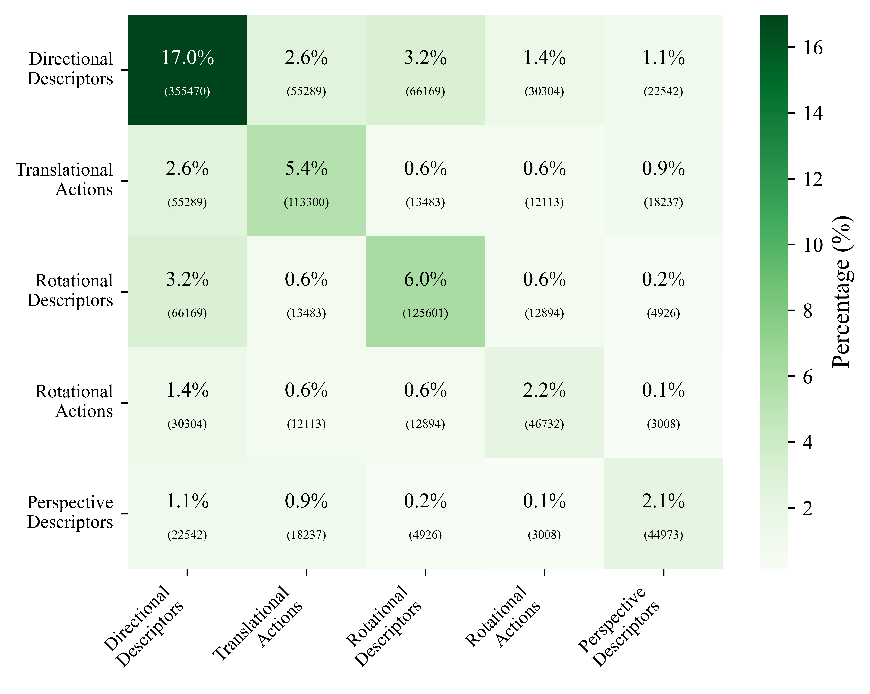
\includegraphics[width=0.5\textwidth]{figures/sft_ds_analysis.pdf}
    \caption{\textbf{Heatmap of Occurances of Spatial-Temporal Terms in popular video SFT datasets.}}
    \label{fig:sft_ds}
\end{figure}

\section{Probing Future Solutions}
To probe promising future solutions for enhancing spatiotemporal video understanding, we propose two approaches that address some of the shortcomings of current state-of-the-art VLMs: fine-tuning a VLM on data-rich in spatiotemporal actions and the other leveraging 4D reconstruction and feature fields jointly with a VLM. SFT refines the model’s abilities by training on datasets that contain temporally and spatially rich actions and interactions. By integrating structured visual representations and targeted fine-tuning, these approaches enhance video-language models’ ability to interpret motion. The second method lifts the feature space of VLMs into a temporally coherent 4D feature field, providing structured scene representations that improve motion and spatial reasoning in the stage of decoding and inference.

\paragraph{Spatial-Temporal SFT}
We evaluate on a subset split of the real dataset by splitting the real-world dataset into a training and testing split (80\% / 20\%) and we try settings using synthetic/real/both for training. We conducted the experiments using Qwen 2VL (7B) and Qwen 2.5VL (7B) through LLama-Factory~\cite{zheng2024llamafactory}, and compared the performance before and after supervised fine-tuning in~\cref{tab:sft}. The results demonstrated an improvement in accuracy in spatiotemporal reasoning, suggesting that performance gains can be obtained through targeted training. However, the addition of synthetic data does not necessarily increase performance over using real data alone, suggesting the importance of synthetic data quality.

% \paragraph{4D Feature Fields Reconstruction}
% Recent advancements in the area of 3D/4D reconstruction, such as Feature4X~\cite{zhou2025feature4x}, have demonstrated notable improvements in VLM performance for visual question answering (VQA) tasks by injecting the 4D scene representation in the feature space at the VLM inference stage. Motivated by these promising results, we explore to inject the spatiotemporal awareness following their 4D feature lifting methodology to evaluate its effectiveness on enhancing the spatiotemporal understanding of the InternVideo2-8B~\cite{wang2024internvideo2} model,testing on the subset of \texttt{VLM4D} including all 50 videos from DAVIS 2016 dataset~\cite{perazzi2016benchmark}. 

% Our experiments involved comparative inference evaluations across three distinct input modalities: original 2D videos, reconstructed global view RGB videos (4D ), and reconstructed global feature fields. As illustrated in Table~\ref{tab:4D_recon_results}, the highest accuracy was consistently obtained using the reconstructed semantic feature fields, highlighting the advantages of structured 4D scene representations. These findings confirm that global 4D feature field reconstruction substantially enriches contextual understanding while bypassing the affect by the artifact from RGB rendering during 4D reconstruction. However, this method is not a generalizable method but a per-scene optimization post-processing method, thereby significantly time-consuming.
% \paragraph{4D Feature Fields Reconstruction}
% Recent advancements in the area of 3D/4D reconstruction, such as Feature4X~\cite{zhou2025feature4x}, have demonstrated notable improvements in VLM performance for visual question answering (VQA) tasks by injecting the 4D scene representation in the feature space at the VLM inference stage. Motivated by these promising results, we explore to inject the spatiotemporal awareness following their 4D feature lifting methodology to evaluate its effectiveness on enhancing the spatiotemporal understanding of the InternVideo2-8B~\cite{wang2024internvideo2} model,testing on the subset of \texttt{VLM4D} including all 50 videos from DAVIS 2016 dataset~\cite{perazzi2016benchmark}. Our experiments involved comparative inference evaluations across three distinct input modalities: original 2D videos, reconstructed global view RGB videos (4D), and reconstructed global 4D feature field. As illustrated in~\cref{tab:4D_recon_results}, the highest accuracy was consistently obtained using the reconstructed semantic feature fields, highlighting the advantages of structured 4D scene representations. These findings confirm that global 4D feature field reconstruction substantially enriches contextual understanding while bypassing the affect by the artifact from RGB rendering during 4D reconstruction. However, this method is not a generalizable method but a per-scene optimization post-processing method, thereby significantly time-consuming.

\paragraph{4D Feature Fields Reconstruction} Recent advances in 3D/4D reconstruction methods, such as Feature4X~\cite{zhou2025feature4x}, have significantly enhanced Vision-Language Model (VLM) performance on visual question answering (VQA) tasks by integrating structured 4D scene representations into the model’s inference stage. Inspired by these promising results, we investigate incorporating spatiotemporal awareness into the InternVideo2-8B model~\cite{wang2024internvideo2}, employing the 4D feature lifting strategy proposed by Feature4X. To assess this approach, we evaluate performance on a subset of the \texttt{VLM4D} benchmark, specifically leveraging all 50 videos from the DAVIS 2016 dataset~\cite{perazzi2016benchmark}.
Our experimental evaluation compares the inference results across three distinct input modalities: original 2D videos, reconstructed global-view RGB videos (4D), and reconstructed global semantic feature fields. As demonstrated in Table~\ref{tab:4D_recon_results}, the highest accuracy consistently results from the reconstructed semantic feature fields, highlighting the clear advantages of structured 4D representations. These findings confirm that global 4D feature field reconstruction enhances contextual understanding and mitigates artifacts associated with RGB rendering during reconstruction. However, the current approach requires per-scene optimization as a post-processing step, limiting its generalizability and making it computationally intensive.

\begin{table}[t]
    \centering
    \renewcommand{\arraystretch}{1.2}
    \begin{tabular}{l|cc}
        \toprule
        \textbf{Model} & \textbf{FF} & \textbf{MC} \\
        \midrule
        \rowcolor[HTML]{e1f0f5} \textit{Original Model} & \phantom{-} & \phantom{-} \\
        Qwen 2VL (7B) & 31.9 & 38.3 \\
        Qwen 2.5VL (7B) & 31.6 & 43.4 \\
        % Video-LLama3 (3B) & - & - \\
        \midrule
        \rowcolor[HTML]{e1f0f5} \textit{Finetuned Model} & & \\
        Qwen 2VL (7B) (R) & \textbf{50.7} & 53.5 \\
        Qwen 2VL (7B) (S) & 38.9 & 41.0 \\
        Qwen 2VL (7B) (R+S) & 49.7 & 52.8 \\
        Qwen 2.5VL (7B) (R) & 48.9 & \textbf{56.3} \\
        Qwen 2.5VL (7B) (S) & 35.4 & 42.0 \\
        Qwen 2.5VL (7B) (R+S) & 39.2 & 48.3 \\
        % Video-LLama3 (3B) (R) & - & - \\
        % Video-LLama3 (3B) (R+S) & - & - \\
        \bottomrule
    \end{tabular}
    \caption{\textbf{SFT on Spatial-Temporal Datasets.} MC and FF refer to multiple-choice and freeform accuracy, respectively. R means SFT using the real-world dataset, S denotes the synthetic dataset, R+S represents using both.}
    \label{tab:sft}
\end{table}

\begin{table}[t]
    \centering
    \renewcommand{\arraystretch}{1.2}
    \begin{tabular}{l|cc}
        \toprule
        \textbf{Input Modality} & \textbf{Accuracy} \\
        \midrule
        \rowcolor[HTML]{e1f0f5} \textit{Chain of Thought Response} & \phantom{-} & \phantom{-} \\
        Original 2D Video & 36.0 \\
        Global View Video & 32.7 \\
        Global Feature Field & \textbf{37.4} \\
        \midrule
        \rowcolor[HTML]{e1f0f5} \textit{Direct Output Response} & & \\
        Original 2D Video & 24.3 \\
        Global View Video & 23.8 \\
        Global Feature Field & \textbf{29.0} \\
        \bottomrule
    \end{tabular}
    \caption{\textbf{InternVideo2 Accuracy with 4D Reconstruction.} Comparison of InternVideo2 accuracy given different input modalities from the same dataset.}
    \label{tab:4D_recon_results}
    \vspace{-0.3cm}
\end{table}

% \begin{table*}[h]
%     \centering
%     \renewcommand{\arraystretch}{1.2}
%     \begin{tabular}{lccc}
%         \toprule
%         \textbf{Model} &  \makecell{\textbf{Synthetic (CoT)}}  & \makecell{\textbf{3rd Person}\\ \textbf{Perspective (CoT)}} &  \makecell{\textbf{1st Person}\\ \textbf{Perspective (CoT)}} \\
%         \midrule
%         \rowcolor[HTML]{F5E8DC} ProLong (8B) & 20.4 / 25.4 & \textbf{28.4} / \textbf{30.1} & 17.0 / 17.1 \\
%         MegaBeam-Mistral (7B) & 512K & 19.8 & \textbf{18.3} \\
%         Meta-Llama-3.1 (8B) & 128K & 17.3 & 16.4 \\
%         Mistral-Nemo (12B) & 128K & 13.6 & 0.4 \\
%         \midrule
%         Jamba-1.5-Mini (12B/52B) & 256K & 27.2 & 28.0 \\
%         Meta-Llama-3.1 (70B) & 128K & 42.0 & 25.0 \\
%         Gemini-1.5-Pro & 2M & 24.7 & 38.8 \\
%         GPT-4o & 128K & 55.6 & 58.4  \\
%         \bottomrule
%     \end{tabular}
%     \caption{\textbf{Big Results Evaluation of Various VLLMs}}
% \end{table*}
\section{Conclusion}
Through the construction of the~\texttt{VLM4D} benchmark, we evaluate the spatiotemporal reasoning capabilities of various Vision-Language Models (both open-source and proprietary). While more recently released models demonstrate improved performance over their counterparts, they remain significantly behind human proficiency. Overall, our work questions whether VLMs posses spatiotemporal reasoning abilities that are imperative to have for more sophisticated visual agents in fields ranging from robotics to interactive AI systems that require a deep understanding of dynamic visual environments. We hope to inspire future work to explore novel approaches for integrating spatiotemporal grounding, thereby enhancing their spatiotemporal reasoning capabilities and facilitating robust deployment. 
\newpage

{
    \small
    \bibliographystyle{ieeenat_fullname}
    \bibliography{main}
}


\end{document}
